%!TEX root = main.tex

\section{SVM Binary Classifier} \label{sec:svm}

We trained a Support Vector Machine (SVM) to do binary classification on local pedestrian trajectories, to predict whether the trajectory will/will not enter a 4x10m rectangle in front of the vehicle.
A portion of the pedestrian trajectory is fed into the classifier, and it outputs a binary label.
This could be a useful safety feature on a car to identify which pedestrians might cross in front of the vehicle.

The trajectories are all of different length, so we split them up into equal ``snippets'' of length $l$.
Each trajectory has a single 0/1 label, and this same label is applied to each snippet.
This allows us to learn some notion of direction from (x,y) sequences, because a snippet that never crosses in front of the vehicle can still be labeled as such, if a later portion of its trajectory eventually does cross in front.
These $l$-long lists of (x,y) points are fed into the classifier as the feature vector of length $2l$, as:
$(x_i = [x_1, y_1, x_2, y_2, ... , x_l, y_l]; y_i = 0/1)$.

We used the SKLearn implementation of SVM~\cite{scikit-learn} with Gaussian RBF Kernel.

\subsection{Simple Example}
We first tried training with $l=1$, so that we could easily visualize the decision boundary in~\cref{fig:svm_snippet1}.
The data (magenta/cyan) aren't particularly meaningful, because it's hard to learn anything from a single (x,y) position of a pedestrian ($l=1$).
But, we can observe that the green decision boundary roughly resembles our arbitrarily-created rectangular ``cross zone''.
This figure indicates the SVM is correctly learning that there is a region in space that causes trajectories to be labeled a certain way.
After this quick sanity check, we can proceed to larger values of $l$, but lose the ability to easily visualize the results.

\begin{figure}
	\centering
	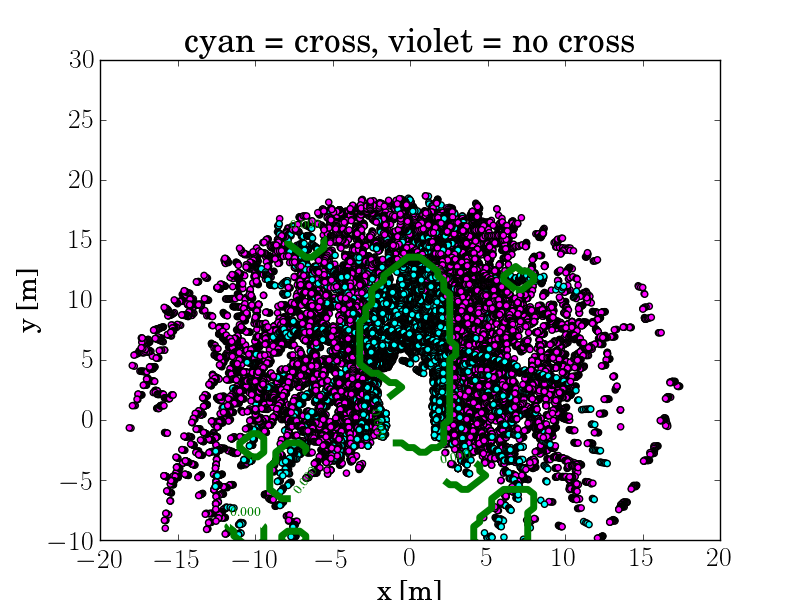
\includegraphics [trim=0 0 0 0, clip, angle=0, width=0.8\columnwidth,
	keepaspectratio]{figures/svm_snippet1}
	\caption{SVM trained on snippets with $l=1$ allow visualization of decision boundary. The important part of this plot is the green decision boundary in the center that resembles our arbitrary ``cross zone''. The SVM has roughly learned the location/shape of zone for simple input data. There is some overfitting evident by other green regions, but this is likely more of an artifact of $l=1$ hyperparameter.} 
	\label{fig:svm_snippet1} 
\end{figure}

\subsection{Hyperparameters}
There are several hyperparameters that affect the behavior of the classifier.
The main ones that we experimented with were $l$ (snippet length) and $C$ (SVM regularizer).
A grid search for optimal parameter values is shown in~\cref{table_svm} (optimal w.r.t. high validation accuracy).

As $C$ increases, training accuracy increases for all scenarios, which is expected because this corresponds to more penalty on mis-classified points.
We can tell when $C$ is too high, because training accuracy is much higher than validation accuracy, a symptom of overfitting.

As $l$ increases, more time steps of pedestrian positions are used in the feature vector, so there is more information on which to classify.
Intuitively, large $l$ would seem preferable than small, but if $l$ is too large, the noise in the data may outweigh the value of the information.
To be more concrete, it seems unlikely that one would need 50 points worth of trajectory data to do the binary classification (especially given the noise seen in~\cref{fig:training_set}).

This intuition aligns with our observed validation accuracies.
The highest validation accuracy of 79.8\% occurs with $l=25$ and $C=10$, so we choose those as the optimal hyperparameters.

The test accuracy with these values was 74.4\%.



\begin{table*}[ht!]
\centering
\begin{tabular}{||c| c c c c c c c| c c c c c c c||}  
 \hline
 \multirow{2}{*}{Dataset} &
       \multicolumn{7}{c|}{$l=2$} &
       \multicolumn{7}{c||}{$l=10$} \\
 & $C=10^{-3}$ & $10^{-2}$ & $10^{-1}$ & $10^{0}$ & $10^{1}$ & $10^{2}$ & $10^{3}$ & $10^{-3}$ & $10^{-2}$ & $10^{-1}$ & $10^{0}$ & $10^{1}$ & $10^{2}$ & $10^{3}$ \\ [0.5ex] 
 \hline\hline
 Train & 70.8 & 83.2 & 84.8 & 85.9 & 87.1 & 89.1 & 91.9 & 63.8 & 76.1 & 84.6 & 86.8 & 92.6 & 97.2 & 99.6  \\ \hline
 Val & 63.1 & 77.4 & 79.1 & 78.9 & 78.0 & 77.8 & 77.6 & 60.3 & 67.9 & 78.4 & 79.4 & 79.3 & 77.7 & 76.1  \\ \hline
\end{tabular}
\begin{tabular}{||c| c c c c c c c| c c c c c c c||}  
 \hline
 \multirow{2}{*}{Dataset} &
       \multicolumn{7}{c|}{$l=25$} &
       \multicolumn{7}{c||}{$l=50$} \\
 & $C=10^{-3}$ & $10^{-2}$ & $10^{-1}$ & $10^{0}$ & $10^{1}$ & $10^{2}$ & $10^{3}$ & $10^{-3}$ & $10^{-2}$ & $10^{-1}$ & $10^{0}$ & $10^{1}$ & $10^{2}$ & $10^{3}$ \\ [0.5ex] 
 \hline\hline
 Train & 62.9 & 64.9 & 82.4 & 88.7 & 96.8 & 99.9 & 100 & 60.4 & 60.4 & 77.6 & 92.2 & 99.3 & 100 & 100  \\ \hline
 Val & 59.2 & 59.3 & 75.0 & 79.7 & 79.8 & 78.8 & 78.8 & 52.3 & 52.3 & 64.8 & 75.0 & 74.8 & 74.5 & 74.5  \\ \hline
\end{tabular}
\caption{Accuracy of SVM for various values of hyperparameters $C$, $l$.}
\label{table_svm}
\end{table*}

\subsection{Results}
With these optimized hyperparameters, we show the various combinations of true/predicted labels in~\cref{fig:svm_labels}.

\begin{table}[ht!]
\centering
\begin{tabular}{||c||c c||}  
 \hline
 Classification & Number & Percent \\
 \hline\hline
 False Positives & 136 & 5.0 \\ \hline
 False Negatives & 554 & 20.4 \\ \hline
 True Positives & 691 & 25.4 \\ \hline
 True Negatives & 1339 & 49.2 \\ \hline\hline
 Total & 2720 & 100.0\\ \hline
\end{tabular}
\caption{Classification matrix}
\label{table_svm_outputs}
\end{table}


\begin{figure}
\centering
\begin{subfigure}{.25\textwidth}
  \centering
  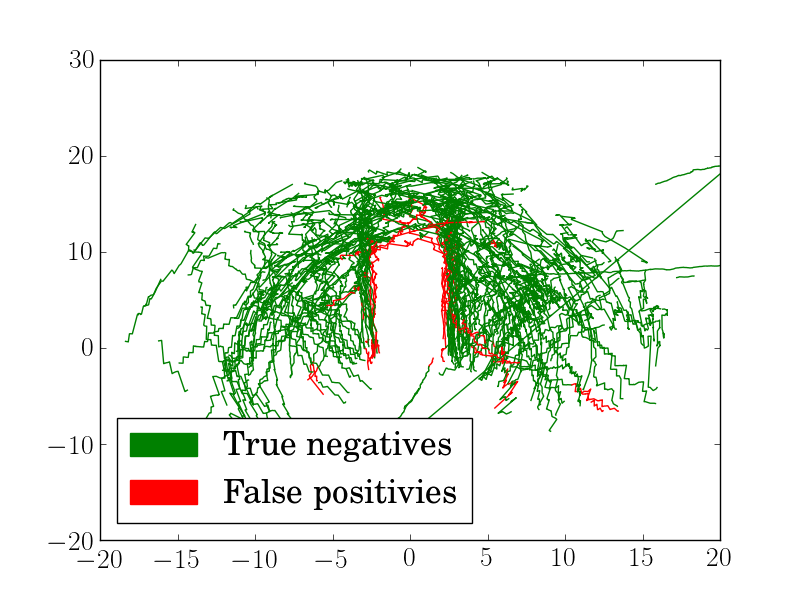
\includegraphics[width=.9\linewidth]{figures/svm_label0}
  \caption{Trajs. labeled "No Cross"}
  \label{fig:svm_label0}
\end{subfigure}%
\begin{subfigure}{.25\textwidth}
  \centering
  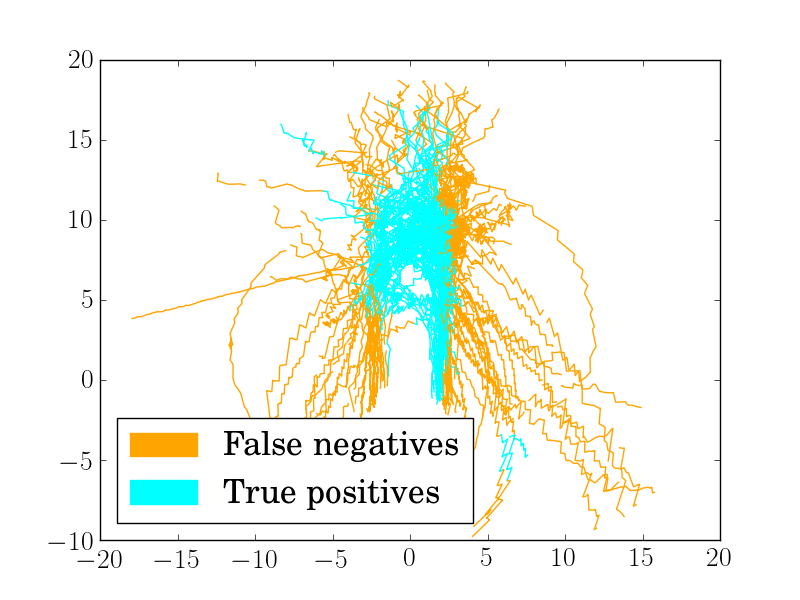
\includegraphics[width=.9\linewidth]{figures/svm_label1}
  \caption{Trajs. labeled "Cross"}
  \label{fig:svm_label1}
\end{subfigure}
\caption{}
\label{fig:svm_labels}
\end{figure}

\meXX{add plot with our trajectories labeled as 0/1}


\subsection{Kernel Choice}
\meXX{discuss kernel options?}


% t_steps: 2, C: 0.001000, Train: 0.708, Val: 0.631, Test: 0.590
% t_steps: 2, C: 0.010000, Train: 0.832, Val: 0.774, Test: 0.724
% t_steps: 2, C: 0.100000, Train: 0.848, Val: 0.791, Test: 0.733
% t_steps: 2, C: 1.000000, Train: 0.859, Val: 0.789, Test: 0.728
% t_steps: 2, C: 10.000000, Train: 0.871, Val: 0.780, Test: 0.721
% t_steps: 2, C: 100.000000, Train: 0.891, Val: 0.778, Test: 0.717
% t_steps: 2, C: 1000.000000, Train: 0.919, Val: 0.776, Test: 0.723

% t_steps: 10, C: 0.001000, Train: 0.638, Val: 0.603, Test: 0.555
% t_steps: 10, C: 0.010000, Train: 0.761, Val: 0.679, Test: 0.643
% t_steps: 10, C: 0.100000, Train: 0.846, Val: 0.784, Test: 0.732
% t_steps: 10, C: 1.000000, Train: 0.868, Val: 0.794, Test: 0.739
% t_steps: 10, C: 10.000000, Train: 0.926, Val: 0.793, Test: 0.736
% t_steps: 10, C: 100.000000, Train: 0.972, Val: 0.777, Test: 0.725
% t_steps: 10, C: 1000.000000, Train: 0.996, Val: 0.761, Test: 0.711

% t_steps: 25, C: 0.001000, Train: 0.629, Val: 0.592, Test: 0.542
% t_steps: 25, C: 0.010000, Train: 0.649, Val: 0.593, Test: 0.546
% t_steps: 25, C: 0.100000, Train: 0.824, Val: 0.750, Test: 0.709
% t_steps: 25, C: 1.000000, Train: 0.887, Val: 0.797, Test: 0.746
% t_steps: 25, C: 10.000000, Train: 0.968, Val: 0.798, Test: 0.744
% t_steps: 25, C: 100.000000, Train: 0.999, Val: 0.788, Test: 0.730
% t_steps: 25, C: 1000.000000, Train: 1.000, Val: 0.788, Test: 0.730

% t_steps: 50, C: 0.001000, Train: 0.604, Val: 0.569, Test: 0.523
% t_steps: 50, C: 0.010000, Train: 0.604, Val: 0.569, Test: 0.523
% t_steps: 50, C: 0.100000, Train: 0.776, Val: 0.676, Test: 0.648
% t_steps: 50, C: 1.000000, Train: 0.922, Val: 0.804, Test: 0.750
% t_steps: 50, C: 10.000000, Train: 0.993, Val: 0.818, Test: 0.748
% t_steps: 50, C: 100.000000, Train: 1.000, Val: 0.808, Test: 0.745
% t_steps: 50, C: 1000.000000, Train: 1.000, Val: 0.808, Test: 0.745
